
%% project-paper-template.tex
%% v1.0
%% Sept, 2021
%% Craig Stewart
%% for Durham University, Computer Science Project paper templates
%% contact craig.d.stewart at durham.ac.uk for support
%%
%% Based on IEEE Template: bare_jrnl_compsoc.tex, V1.4b, by Michael Shell
%%
%% Notice from original IEEE Template:
%%*************************************************************************
%% Legal Notice:
%% This code is offered as-is without any warranty either expressed or
%% implied; without even the implied warranty of MERCHANTABILITY or
%% FITNESS FOR A PARTICULAR PURPOSE! 
%% User assumes all risk.
%% In no event shall the IEEE or any contributor to this code be liable for
%% any damages or losses, including, but not limited to, incidental,
%% consequential, or any other damages, resulting from the use or misuse
%% of any information contained here.
%%
%% All comments are the opinions of their respective authors and are not
%% necessarily endorsed by the IEEE.
%%
%% This work is distributed under the LaTeX Project Public License (LPPL)
%% ( http://www.latex-project.org/ ) version 1.3, and may be freely used,
%% distributed and modified. A copy of the LPPL, version 1.3, is included
%% in the base LaTeX documentation of all distributions of LaTeX released
%% 2003/12/01 or later.
%% Retain all contribution notices and credits.
%% ** Modified files should be clearly indicated as such, including  **
%% ** renaming them and changing author support contact information. **
%%*************************************************************************


\documentclass[10pt,journal,compsoc]{IEEEtran}

% Some very useful LaTeX packages include:
% (uncomment the ones you want to load)


%% ---------------------------------------------- START OF USEFUL PACKAGES ----------------------------------------------

%\usepackage{ifpdf}
% Heiko Oberdiek's ifpdf.sty is very useful if you need conditional
% compilation based on whether the output is pdf or dvi.
% usage:
% \ifpdf
%   % pdf code
% \else
%   % dvi code
% \fi
% The latest version of ifpdf.sty can be obtained from:
% http://www.ctan.org/pkg/ifpdf
% Also, note that IEEEtran.cls V1.7 and later provides a builtin
% \ifCLASSINFOpdf conditional that works the same way.
% When switching from latex to pdflatex and vice-versa, the compiler may
% have to be run twice to clear warning/error messages.


% *** CITATION PACKAGES ***
%
\ifCLASSOPTIONcompsoc
  % IEEE Computer Society needs nocompress option
  % requires cite.sty v4.0 or later (November 2003)
  \usepackage[nocompress]{cite}
\else
  % normal IEEE
  \usepackage{cite}
\fi

% cite.sty was written by Donald Arseneau
% V1.6 and later of IEEEtran pre-defines the format of the cite.sty package
% \cite{} output to follow that of the IEEE. Loading the cite package will
% result in citation numbers being automatically sorted and properly
% "compressed/ranged". e.g., [1], [9], [2], [7], [5], [6] without using
% cite.sty will become [1], [2], [5]--[7], [9] using cite.sty. cite.sty's
% \cite will automatically add leading space, if needed. Use cite.sty's
% noadjust option (cite.sty V3.8 and later) if you want to turn this off
% such as if a citation ever needs to be enclosed in parenthesis.
% cite.sty is already installed on most LaTeX systems. Be sure and use
% version 5.0 (2009-03-20) and later if using hyperref.sty.
% The latest version can be obtained at:
% http://www.ctan.org/pkg/cite
% The documentation is contained in the cite.sty file itself.
%
% Note that some packages require special options to format as the Computer
% Society requires. In particular, Computer Society  papers do not use
% compressed citation ranges as is done in typical IEEE papers
% (e.g., [1]-[4]). Instead, they list every citation separately in order
% (e.g., [1], [2], [3], [4]). To get the latter we need to load the cite
% package with the nocompress option which is supported by cite.sty v4.0
% and later. Note also the use of a CLASSOPTION conditional provided by
% IEEEtran.cls V1.7 and later.


% *** GRAPHICS RELATED PACKAGES ***
%
\ifCLASSINFOpdf
  \usepackage[pdftex]{graphicx}
  % declare the path(s) where your graphic files are
  % \graphicspath{{../pdf/}{../jpeg/}}
  % and their extensions so you won't have to specify these with
  % every instance of \includegraphics
  % \DeclareGraphicsExtensions{.pdf,.jpeg,.png}
\else
  % or other class option (dvipsone, dvipdf, if not using dvips). graphicx
  % will default to the driver specified in the system graphics.cfg if no
  % driver is specified.
  % \usepackage[dvips]{graphicx}
  % declare the path(s) where your graphic files are
  % \graphicspath{{../eps/}}
  % and their extensions so you won't have to specify these with
  % every instance of \includegraphics
  % \DeclareGraphicsExtensions{.eps}
\fi
% graphicx was written by David Carlisle and Sebastian Rahtz. It is
% required if you want graphics, photos, etc. graphicx.sty is already
% installed on most LaTeX systems. The latest version and documentation
% can be obtained at: 
% http://www.ctan.org/pkg/graphicx
% Another good source of documentation is "Using Imported Graphics in
% LaTeX2e" by Keith Reckdahl which can be found at:
% http://www.ctan.org/pkg/epslatex
%
% latex, and pdflatex in dvi mode, support graphics in encapsulated
% postscript (.eps) format. pdflatex in pdf mode supports graphics
% in .pdf, .jpeg, .png and .mps (metapost) formats. Users should ensure
% that all non-photo figures use a vector format (.eps, .pdf, .mps) and
% not a bitmapped formats (.jpeg, .png). The IEEE frowns on bitmapped formats
% which can result in "jaggedy"/blurry rendering of lines and letters as
% well as large increases in file sizes.
%
% You can find documentation about the pdfTeX application at:
% http://www.tug.org/applications/pdftex


% *** MATH PACKAGES ***
%
%\usepackage{amsmath}
% A popular package from the American Mathematical Society that provides
% many useful and powerful commands for dealing with mathematics.
%
% Note that the amsmath package sets \interdisplaylinepenalty to 10000
% thus preventing page breaks from occurring within multiline equations. Use:
%\interdisplaylinepenalty=2500
% after loading amsmath to restore such page breaks as IEEEtran.cls normally
% does. amsmath.sty is already installed on most LaTeX systems. The latest
% version and documentation can be obtained at:
% http://www.ctan.org/pkg/amsmath


% *** SPECIALIZED LIST PACKAGES ***
%
%\usepackage{algorithmic}
% algorithmic.sty was written by Peter Williams and Rogerio Brito.
% This package provides an algorithmic environment fo describing algorithms.
% You can use the algorithmic environment in-text or within a figure
% environment to provide for a floating algorithm. Do NOT use the algorithm
% floating environment provided by algorithm.sty (by the same authors) or
% algorithm2e.sty (by Christophe Fiorio) as the IEEE does not use dedicated
% algorithm float types and packages that provide these will not provide
% correct IEEE style captions. The latest version and documentation of
% algorithmic.sty can be obtained at:
% http://www.ctan.org/pkg/algorithms
% Also of interest may be the (relatively newer and more customizable)
% algorithmicx.sty package by Szasz Janos:
% http://www.ctan.org/pkg/algorithmicx


% *** ALIGNMENT PACKAGES ***
%
%\usepackage{array}
% Frank Mittelbach's and David Carlisle's array.sty patches and improves
% the standard LaTeX2e array and tabular environments to provide better
% appearance and additional user controls. As the default LaTeX2e table
% generation code is lacking to the point of almost being broken with
% respect to the quality of the end results, all users are strongly
% advised to use an enhanced (at the very least that provided by array.sty)
% set of table tools. array.sty is already installed on most systems. The
% latest version and documentation can be obtained at:
% http://www.ctan.org/pkg/array


% IEEEtran contains the IEEEeqnarray family of commands that can be used to
% generate multiline equations as well as matrices, tables, etc., of high
% quality.


% *** SUBFIGURE PACKAGES ***
%\ifCLASSOPTIONcompsoc
%  \usepackage[caption=false,font=footnotesize,labelfont=sf,textfont=sf]{subfig}
%\else
%  \usepackage[caption=false,font=footnotesize]{subfig}
%\fi
% subfig.sty, written by Steven Douglas Cochran, is the modern replacement
% for subfigure.sty, the latter of which is no longer maintained and is
% incompatible with some LaTeX packages including fixltx2e. However,
% subfig.sty requires and automatically loads Axel Sommerfeldt's caption.sty
% which will override IEEEtran.cls' handling of captions and this will result
% in non-IEEE style figure/table captions. To prevent this problem, be sure
% and invoke subfig.sty's "caption=false" package option (available since
% subfig.sty version 1.3, 2005/06/28) as this is will preserve IEEEtran.cls
% handling of captions.
% Note that the Computer Society format requires a sans serif font rather
% than the serif font used in traditional IEEE formatting and thus the need
% to invoke different subfig.sty package options depending on whether
% compsoc mode has been enabled.
%
% The latest version and documentation of subfig.sty can be obtained at:
% http://www.ctan.org/pkg/subfig


% *** FLOAT PACKAGES ***
%
%\usepackage{fixltx2e}
% fixltx2e, the successor to the earlier fix2col.sty, was written by
% Frank Mittelbach and David Carlisle. This package corrects a few problems
% in the LaTeX2e kernel, the most notable of which is that in current
% LaTeX2e releases, the ordering of single and double column floats is not
% guaranteed to be preserved. Thus, an unpatched LaTeX2e can allow a
% single column figure to be placed prior to an earlier double column
% figure.
% Be aware that LaTeX2e kernels dated 2015 and later have fixltx2e.sty's
% corrections already built into the system in which case a warning will
% be issued if an attempt is made to load fixltx2e.sty as it is no longer
% needed.
% The latest version and documentation can be found at:
% http://www.ctan.org/pkg/fixltx2e

%\usepackage{stfloats}
% stfloats.sty was written by Sigitas Tolusis. This package gives LaTeX2e
% the ability to do double column floats at the bottom of the page as well
% as the top. (e.g., "\begin{figure*}[!b]" is not normally possible in
% LaTeX2e). It also provides a command:
%\fnbelowfloat
% to enable the placement of footnotes below bottom floats (the standard
% LaTeX2e kernel puts them above bottom floats). This is an invasive package
% which rewrites many portions of the LaTeX2e float routines. It may not work
% with other packages that modify the LaTeX2e float routines. The latest
% version and documentation can be obtained at:
% http://www.ctan.org/pkg/stfloats
% Do not use the stfloats baselinefloat ability as the IEEE does not allow
% \baselineskip to stretch. Authors submitting work to the IEEE should note
% that the IEEE rarely uses double column equations and that authors should try
% to avoid such use. Do not be tempted to use the cuted.sty or midfloat.sty
% packages (also by Sigitas Tolusis) as the IEEE does not format its papers in
% such ways.
% Do not attempt to use stfloats with fixltx2e as they are incompatible.
% Instead, use Morten Hogholm'a dblfloatfix which combines the features
% of both fixltx2e and stfloats:
%
% \usepackage{dblfloatfix}
% The latest version can be found at:
% http://www.ctan.org/pkg/dblfloatfix


%\ifCLASSOPTIONcaptionsoff
%  \usepackage[nomarkers]{endfloat}
% \let\MYoriglatexcaption\caption
% \renewcommand{\caption}[2][\relax]{\MYoriglatexcaption[#2]{#2}}
%\fi
% endfloat.sty was written by James Darrell McCauley, Jeff Goldberg and 
% Axel Sommerfeldt. This package may be useful when used in conjunction with 
% IEEEtran.cls'  captionsoff option. Some IEEE journals/societies require that
% submissions have lists of figures/tables at the end of the paper and that
% figures/tables without any captions are placed on a page by themselves at
% the end of the document. If needed, the draftcls IEEEtran class option or
% \CLASSINPUTbaselinestretch interface can be used to increase the line
% spacing as well. Be sure and use the nomarkers option of endfloat to
% prevent endfloat from "marking" where the figures would have been placed
% in the text. The two hack lines of code above are a slight modification of
% that suggested by in the endfloat docs (section 8.4.1) to ensure that
% the full captions always appear in the list of figures/tables - even if
% the user used the short optional argument of \caption[]{}.
% IEEE papers do not typically make use of \caption[]'s optional argument,
% so this should not be an issue. A similar trick can be used to disable
% captions of packages such as subfig.sty that lack options to turn off
% the subcaptions:
% For subfig.sty:
% \let\MYorigsubfloat\subfloat
% \renewcommand{\subfloat}[2][\relax]{\MYorigsubfloat[]{#2}}
% However, the above trick will not work if both optional arguments of
% the \subfloat command are used. Furthermore, there needs to be a
% description of each subfigure *somewhere* and endfloat does not add
% subfigure captions to its list of figures. Thus, the best approach is to
% avoid the use of subfigure captions (many IEEE journals avoid them anyway)
% and instead reference/explain all the subfigures within the main caption.
% The latest version of endfloat.sty and its documentation can obtained at:
% http://www.ctan.org/pkg/endfloat
%
% The IEEEtran \ifCLASSOPTIONcaptionsoff conditional can also be used
% later in the document, say, to conditionally put the References on a 
% page by themselves.


% *** PDF, URL AND HYPERLINK PACKAGES ***
%
%\usepackage{url}
% url.sty was written by Donald Arseneau. It provides better support for
% handling and breaking URLs. url.sty is already installed on most LaTeX
% systems. The latest version and documentation can be obtained at:
% http://www.ctan.org/pkg/url
% Basically, \url{my_url_here}.

%% ---------------------------------------------- END OF USEFUL PACKAGES ----------------------------------------------



% *** Do not adjust lengths that control margins, column widths, etc. ***
% *** Do not use packages that alter fonts (such as pslatex).         ***

% correct bad hyphenation here
\hyphenation{op-tical net-works semi-conduc-tor}

\begin{document}
%
% paper title
% Titles are generally capitalized except for words such as a, an, and, as,
% at, but, by, for, in, nor, of, on, or, the, to and up, which are usually
% not capitalized unless they are the first or last word of the title.
% Linebreaks \\ can be used within to get better formatting as desired.
% Do not put math or special symbols in the title.
\title{Building a Fair Online Casino on the Blockchain}
%
%
% author  

\author{Student Name: Adam Hodson\\Supervisor Name:  Dr. Ioannis Ivrissimtzis\\
Submitted as part of the degree of BSc Computer Science to the\\
Board of Examiners in the Department of Computer Sciences, Durham University
}


% The paper headers
\markboth{DURHAM UNIVERSITY, DEPARTMENT OF COMPUTER SCIENCE}%
{Shell \MakeLowercase{\textit{et al.}}}

\IEEEtitleabstractindextext{%
\begin{abstract}
%These instructions give you guidelines for preparing your project report. DO NOT change any settings, such as margins and %font sizes. Just use this as a template and modify the contents into your final paper. An abstract should be 100 to 200 %words, and should clearly state the nature and significance of the paper. Abstracts must not include mathematical %expressions or bibliographic references. Please note that abstracts are formatted as left justified in our editing %template (as shown here).
TODO ac tortor vitae purus faucibus ornare suspendisse sed nisi lacus sed viverra tellus in hac habitasse platea dictumst vestibulum rhoncus est pellentesque elit ullamcorper dignissim cras tincidunt lobortis feugiat vivamus at augue eget arcu dictum varius duis at consectetur lorem donec massa sapien faucibus et molestie ac feugiat sed lectus vestibulum mattis ullamcorper velit sed ullamcorper morbi tincidunt ornare massa eget egestas purus viverra accumsan in nisl nisi scelerisque eu ultrices vitae auctor eu augue ut lectus arcu bibendum at varius vel pharetra vel turpis nunc eget lorem dolor sed viverra ipsum nunc aliquet bibendum enim facilisis gravida neque convallis a cras semper auctor neque vitae tempus quam pellentesque nec nam aliquam sem et tortor consequat id porta nibh venenatis cras sed felis eget velit aliquet sagittis id consectetur purus ut faucibus pulvinar elementum integer enim neque volutpat ac tincidunt vitae semper quis lectus nulla at volutpat diam ut venenatis
\end{abstract}

\begin{IEEEkeywords}
% Find more here https://ieeecs-media.computer.org/assets/pdf/taxonomy.pdf
Games, Centralization/decentralization
\end{IEEEkeywords}}

%% --------------------------------------------- DO NOT CHANGE ---------------------------------------------

% make the title area
\maketitle


% To allow for easy dual compilation without having to reenter the
% abstract/keywords data, the \IEEEtitleabstractindextext text will
% not be used in maketitle, but will appear (i.e., to be "transported")
% here as \IEEEdisplaynontitleabstractindextext when the compsoc 
% or transmag modes are not selected <OR> if conference mode is selected 
% - because all conference papers position the abstract like regular
% papers do.
\IEEEdisplaynontitleabstractindextext
% \IEEEdisplaynontitleabstractindextext has no effect when using
% compsoc or transmag under a non-conference mode.
% For peer review papers, you can put extra information on the cover
% page as needed:
% \ifCLASSOPTIONpeerreview
% \begin{center} \bfseries EDICS Category: 3-BBND \end{center}
% \fi
%
% For peerreview papers, this IEEEtran command inserts a page break and
% creates the second title. It will be ignored for other modes.
\IEEEpeerreviewmaketitle

\IEEEraisesectionheading{\section{Introduction}\label{sec:introduction}}
% Computer Society journal (but not conference!) papers do something unusual
% with the very first section heading (almost always called "Introduction").
% They place it ABOVE the main text! IEEEtran.cls does not automatically do
% this for you, but you can achieve this effect with the provided
% \IEEEraisesectionheading{} command. Note the need to keep any \label that
% is to refer to the section immediately after \section in the above as
% \IEEEraisesectionheading puts \section within a raised box.

%% --------------------------------------------- DO NOT CHANGE ---------------------------------------------
\IEEEPARstart{T}{HE} applications of blockchain are now far beyond scope of an “electronic cash system” proposed in Nakamoto's\cite{Nakamoto2008} seminal paper on blockchain; Bitcoin. Recent interest now lies in how classical, centralized systems can be moved to incorporate blockchain.

This work considers one of the practical applications of blockchain as a replacement for the status quo in the industry of internet-based chance games (iGaming). 

In doing so we aim to answer the following questions; how viable or practical is it to implement a blockchain-backed online casino? Furthermore, to what degree can said implementation leverage the benefits offered by such technologies (i.e. provability, decentralization and security)?
\subsection{Issues with Modern iGaming}
\label{sec:problems}
Traditionally, the only thing stopping a casino (online or physical) from cheating the player is its own reputation, as casinos that cheat will lose business. Online casinos can conceal this cheating as their games run on centralized servers where the user will only ever see the outcome of the game. This is not the case with a blockchain-based platform thus giving even a new platform instant-legitimacy and creating a viable alternative to much disliked giants of the iGaming industry. 

The industry currently suffers from distrust due to centralization of the games themselves, with 45.5\% of users complaining about ‘unfair software’, 59.1\% complaining about not being paid properly and, 25.8\% ‘not being paid at all’ \cite{Gainsbury2013}. 

These alarmingly high rates all point to the vendor scamming the user like in the case of non-payment or that users feel the vendor is scamming them. While this is a common worry amongst gamblers due to the inherent black box nature of online casinos, it is often not the case as large online casinos are heavily regulated in the countries they operate in.

However, the feelings of being cheated are not quelled with promises of auditing. Users prefer to 'see it to believe it'. A blockchain-backed iGaming solution offers a complete solution to this issue as well as the non-payment issue. To explain how this works, some background on decentralized apps must be covered first.
\subsection{An Overview of Blockchain}
\label{sec:introtobloc}
First we must establish an understanding of blockchain as an idea. Fundamentally, a blockchain is a chronological, write-only ledger of transactions. In the simplest form these transactions are simply moving arbitrary tokens from one wallet/user/address to another.

Transactions are grouped into 'blocks' with a unique identifier in the form of a hash determined when adding the block to the network. Transactions in a block are hashed in a Merkle tree \cite{haber1997secure, massias1999design, merkle2019protocols}. Merkle trees have the ideal property wherein the hash of its root node will encode the data of all child nodes, all the way down to the leaves.

For a new block of transactions to be added to the chain, it must first be 'mined'. To mine a block; the miner (a node running the blockchain software) aims to fill in a nonce (number used once) of the given block, shown in \ref{fig:blockdiagram}. This is done by constantly incrementing said nonce by 1, starting from 0, placing it in the nonce slot of the block and hashing it. This resultant hash value is compared with the difficulty value set globally in the software ran by all nodes. If the resultant value is lower than the difficulty then the block is solved.

\begin{figure}[!h]
    \centering
    \includegraphics[width=2in]{figures/BitcoinBlocks.drawio.pdf}
    \caption{The core anatomy of a block, originally proposed for use in Bitcoin \cite{Nakamoto2008}.}
    \label{fig:blockdiagram}
\end{figure}

Next, the network must reach a consensus that this solution is valid. The first proposed, and still most commonly used consensus protocol among blockchains is Proof-of-Work (PoW) \cite{Gervais2016}. A miner with a valid solution will propagate their proposed solution throughout the network as to avoid reliance on a trusted party \cite{dai_1998}. Each node gets one vote on its validity, checking for issues like unsigned transactions, double-spending or improper nonce proposals.

If a majority consensus of block validity is reached then all agreeing nodes with append this to the end of their chain and uses its hash in attempting to mine the next block. From this it is obvious that the longest, validated chain on the network is the source of truth.

In the case of networks like Bitcoin, the miner who submitted a valid block for verification first will be rewarded with a fixed amount of cryptocurrency.

Miners often pool their computing power due to the 'winner takes all' nature of block rewards \cite{etherscan, ethermine}. Others simply buy/rent vast amounts of computing power to consistently beat out competing miners. 

This is a key issue addressed with other consensus protocols like Proof-of-Stake (PoS) where miners (validators) who stake more of the primary cryptocurrency of the network can probabilistically mine (validate) blocks more often than those who have staked less. Thus eliminating the profit incentive driving the compute-power arms-race which consumes huge amounts of energy every year \cite{Li2019}.

\subsection{Second Generation Blockchains}
Second generation blockchains like Ethereum took the core idea of first-generation networks like Bitcoin and introduced the concept of smart contracts\cite{Buterin2014} and the Ethereum Virtual Machine (EVM). These allows Ethereum transactions to do much more than simply move funds like Bitcoin. Understanding the core concepts of Ethereum are integral to understanding all DApps (decentralised applications) \cite{Cai2018} including the work we present.

The first of these concepts; smart contracts, are arbitrary computer programs that anyone can deploy to the blockchain. They can store data on the persistent state of the blockchain. They also offer signed transactions to 'write' to the contract which can perform calculations, operations and modify the persistent state.

Anyone can deploy a smart contract with their own code, interact with it on-chain and read completely deterministic, validated results from it in a trustless decentralized network with no single point of failure \cite{antonopoulos2018mastering} like a 'trusted' authority or server. 

Deploying a smart contract is a special transaction of its own. Once deployed, its code is immutable and persistent between all transactions. It is identified by a unique address like any other user of the blockchain.

The second of these concepts; the EVM, is a classic stack-based machine that operates the same as a Turing machine. This Turing machine however has a very expensive tape as writing values to the persistent state of the blockchain costs a lot of gas. However, writing to the memory is very cheap as it is volatile and not maintained between transactions. 

An instance of the EVM runs on each node on the Ethereum network at all times allowing for the hot-swapping of smart contract states to process validity and reach a consensus on the validity of a mined block (much the same as explained in Section \ref{sec:introtobloc}).

\begin{figure}[!h]
    \centering
    \includegraphics[width=2.5in]{figures/EvmDiagram.drawio.pdf}
    \caption{The structure of the EVM (adapted from EVM illustrated \cite{tani_2018}).}
    \label{fig:evmdiagram}
\end{figure}

This powerful concept has countless possible applications that are only just beginning to be explored by allowing developers to leverage the transparency, immutability and cryptographic security explained in Section \ref{sec:introtobloc} to build arbitrary, trustworthy software.

To interact with the contract a user can perform two types of transactions on it. Firstly there are 'view' interactions where the user wants to query the current state of the contract. These consume gas but the caller does not pay it. Next there is write interactions where the transaction will change the state stored by the contract. These require the transaction to be signed with the invoker's private key to verify the identity of the caller. This allows contracts to store per-user information or change its behaviour depending on the caller.

\subsection{Gas Fees and Transaction Speeds}
All current smart contract-compatible blockchains rely on two things: the concept of gas and a primary (gas) token. For example, ETH is the primary token of the Ethereum network. Gas is a way of measuring how much computational power a particular operation will consume. This could be the transfer of a token from one address to another, deploying a smart contract or interacting (view/write) with a smart contract as covered earlier. The invoker of the transaction will pay a certain amount of the network's primary token to perform their transaction on the network. The amount paid is defined by the fee schedule of the network.

Before signing a transaction and sending it to the network a user will attach a gas limit which acts as an upper bound for how much gas they wish to use. If their transaction exceeds this limit it will revert and the state of the network will not change. They also specify how much they are willing to pay for each unit of gas. For example, the upper limit say a user sends $\theta$ ETH to their friend. This costs 21,000 gas so they would lose $21000 * G_{\textit{fee}} + \theta$ ETH from their wallet while their friend would gain just $\theta$ ETH once the transaction is validated. 

Gas prices fluctuate wildly especially if you care about your transaction being completed in a timely manner. Most modern user wallets will have a built in gas estimator and current gas price tracker for reasonable speed. 

\begin{figure}[!h]
    \centering
    \includegraphics[width=3.5in]{figures/EthGasGraph.png}
    \caption{Ethereum main network daily mean gas fee beginning in 2021 with a 30-day moving average (in wei). This highlights just how volatile unbounded gas prices can be even averaged over an entire 24 hours. Note that 1 wei $ = 1*10^{-18}$ ETH.}
    \label{fig:ethgas}
\end{figure}

Ethereum was not built with scalability in mind and constantly faces severe congestion causing low transaction throughput and high gas fees. These two issues exacerbate one another as users will bid each other up on gas fees to have their transaction processed first due to the slow speed of the network, meaning users are constantly sending new transactions slowing the network down further. 

As a result, Ethereum has an impractically low transaction rate of ~15 TPS (transactions processed per second). Bitcoin, as a comparison, can only manage ~6 TPS. For reference a centralized payment provider like Visa can handle ~24,000 TPS. 

This severely limits the practical applications of Ethereum in real-time or near real-time applications like iGaming. The upcoming 2.0 upgrade should help to fix these issues but for now, many DApp developers are looking towards alternatives.
\subsection{Objectives}
\label{sec:objectives}
In this work, we build a DApp; GlassCasino. This platform allows users to play single and multi-player casino games like Roulette and Chuck-a-Luck \cite{Chuckaluck} which run entirely on a blockchain to leverage the numerous aforementioned  benefits.

Our objectives for achieving this are as follows:
\begin{enumerate}
    \item Implement a small selection of traditional casino games as smart contracts
    \item Integrate verifiable, decentralized randomness into at least one game
    \item Build a robust migration chain to deploy our smart contracts to any compatible network
    \item Construct a cloud-based, always-online client to operate flow of games where necessary
    \item Create a user-friendly, responsive web-based user interface (UI) to play and watch games take place
    \item Add wide-scale standard wallet integration allowing users to play with just a few clicks
    \item Include links to mined blocks and transaction records to allow auditing of games
\end{enumerate}

\subsection{Achievements}
We largely achieved what we set out to do with a key few stipulations that arose during development. Our full achievements are as follows:
\begin{enumerate}
    \item Implemented a multi-player, synchronised traditional roulette game with a small selection of bet types as a smart contract (objective 1)
    \item Implemented a single-player, verifiably random Chuck-a-Luck game as a smart contract (objective 2)
    \item Built out a recorded history of all games recorded on the blockchain via querying event logs (part of objectives 1 and 5)
    \item Designed and built a central bank smart contract that works with any compatible deployed game (part of objective 1)
    \item Integrated roles-based permissions to allow for the introduction of new during development and role renunciation to enforce trustlessness by removing a central point of failure (part of objective 1)
    \item Created a user-friendly, responsive web-based user interface with full wallet integration and complete state management allowing for quick switching between different games (objective 5)
    \item Construction of a cloud-based, always-online client to operate the roulette wheel and synchronise low importance game timing data with the web app (objective 4)
    \item Included links to mined blocks and transaction records on a standard block explorer website (objective 7)
\end{enumerate}

Some key achievements to highlight are numbers 4, 5, and 6.

Achievements 4 and 5 were the result of a challenge that presented itself when developing our second game. This was the concept of banking in the context of a casino. All casinos run a simple banking system in the form of chips. The key tenet of this is they have the ability to have more chips on the floor of the casino than they have actual money in their vaults. 

This means they can pay out any wager in chips even if they haven't made a lot of profit recently and simply tell the player to redeem their chips for cash later. The technical solution to this is presented in Section \ref{sec:bank}.

Achievement 6 involved working with a large technology stack and combining a lot of moving pieces together; smart contracts status, wallet integration, connection to the house server, state management, and responsive design.
\section{Related Work}
The following sections will now introduce the technologies and theories that make this work possible. This includes modern blockchain architectures, verifiable randomness, caveats with other proposed solutions, and other work similar to ours.
\label{sec:related}
\subsection{Plasma \& Polygon}
\label{sec:polygon}
Plasma \cite{Poon2017} is a framework for building level 2 blockchain scaling solutions (L2). In essence, a Plasma chain runs on top of an existing blockchain (referred to as the 'rootchain') so that one does not need to create transactions on the rootchain for every single transaction on the Plasma chain. These chains are often called level 2 chains (L2) or L2 scaling solutions.

\begin{figure}[!h]
    \centering
    \includegraphics[width=3.2in]{figures/PlasmaDiagram.drawio.pdf}
    \caption{Relationship between a Plasma-based L2 chain and its rootchain \cite{Poon2017}.}
    \label{fig:plasma}
\end{figure}

All this is to say, a Plasma-based blockchain like Polygon will have much lower gas fees while maintaining the same security and decentralisation benefits as state updates are validated in bulk by the root network (in this case, Ethereum). Secondly, transaction bandwidth will be considerably higher as minimal data is being passed down to the overloaded Ethereum network. 

It does not disclose the contents of the Plasma chain to the rootchain, instead only block hashes are submitted by Plasma validators utilizing proof of stake consensus. If there is proof of fraud on the root chain, i.e., the block, cannot be validated by the Ethereum network, the block on the Plasma chain will be rolled back and its creator penalized via deducting some of their stake.

Polygon \cite{Kanani2021} uses an adapted version of the Plasma framework to enable secure off-chain smart contracts and transactions that will still eventually be validated by a reliable root blockchain (in Polygon's case; Ethereum). 

Thus, it provides the speed and throughput of a mid-tier centralized system with the security of Ethereum’s vast network of validators. All while providing complete interoperability available with the Ethereum network in that any token on the Ethereum network can be exchange one-to-one with the same token on the Polygon network.
\subsection{ChainLink VRF}
\label{sec:chainlink}
ChainLink \cite{breidenbach2021chainlink} VRF is a provably fair and verifiable source of randomness designed for use in smart contracts. It implements Goldberg’s Verifiable Random Function \cite{cryptoeprint:2017:099} using external oracle nodes with on-chain proof validator smart contracts.

This was previously impossible to do on-chain while being tamper-proof as older methods like using block hash or timestamp to seed a pseudo-random number generator are vulnerable to attacks from miners via withholding mined blocks to change the outcome of a game \cite{Piasecki_2016}. 
Every random number provided by the ChainLink oracle comes with a cryptographic proof to verify its randomness and this proof is verified on-chain before the number is consumed by the smart contract. It is based on elliptic curve cryptography using the secp256k1 curve \cite{sec20002} and Keccak \cite{10.1007/978-3-642-38348-9_19} hashing. 

Keccak is the de-facto standard hash function on the majority of modern blockchains due to its practically zero chance of collisions and ability to accept an infinite input space. For our purposes we simply treat it as a black box accepting any data as input and returning a 256-bit unique, positive integer as output.

\begin{figure}[!h]
    \centering
    \includegraphics[width=1.3in]{figures/ChainLinkVRFDiagram.drawio.pdf}
    \caption{Flowchart demonstrating the process of getting a verifiable random number on the blockchain.}
    \label{fig:chainlinkflow}
\end{figure}

ChainLink maintains a number of oracles nodes each with a secret key $k$ and a public key $pk$ where $p$ is the field of of the secp256k1 curve. This public key is published on-chain.

To generate a random number and its proof, the oracle uses its public key and unpredictable block data (i.e. the next $n$ block headers) as inputs to keccak256 this is the seed $S$. A standard value for $n$ is 10. It repeatedly hashes $S$ until it is less than $p$. This is then taken as the $x$ coordinate of some point on the secp256k1 curve.

Next, it defines the following, where $V$ (when hashed with keccak256) represents our random value. 
\begin{equation}
    V = (x, y) * k
\end{equation}

To build the proof of randomness first the oracle samples a random nonce $n$ in the range $[0, \textit{\#secp256k1-1}]$. Next it computes the following values:
\begin{equation}
    u = \textit{address}(n * g) : g = G_{\textit{secp256k1}}
\end{equation}
\begin{equation}
    v = n * (x, y)
\end{equation}
\begin{equation}
    c = \textit{keccak256}((x, y), pk, V, u, v) \pmod{\textit{\#secp256k1}} 
\end{equation}
\begin{equation}
    s = n - c * k \pmod{\textit{\#secp256k1}} 
\end{equation}
The proof is then defined as the tuple $(pk, V, c, s, S)$ which is sent to an on-chain contract to verify and if it succeeds, will proceed in sending the value $V$ to the consuming smart contract.

This technology is integral to writing any contract that relies on non-deterministic behavior i.e., the roll of a die, or the spin of a roulette wheel. To call the VRF the contract must pay some LINK token depending on which chain it was called from. 

For example, on the Ethereum network it costs 2 LINK (an Ethereum-based token to cover gas fees/ChainLink’s running cost) per VRF call ($\sim$60 USD as of 30/10/2021) whereas on Polygon it costs 0.0001 LINK ($\sim$0.00301 USD as of 30/10/2021). 

\subsection{Avalanche}
Avalanche is a high-performance, scalable, customizable, and secure blockchain platform \cite{Sekniqi2020} built from the ground up (unlike Polygon). It introduces a new consensus protocol family called Snow \cite{Rocket2019}, which is part of a family of leaderless Byzantine fault tolerance protocols. This new consensus protocol is also very secure and even resilient to a 51\% attack unlike traditional PoW. Avalanche implements such a protocol under the name Snowman.

It is the current fastest standalone smart contract platform available for use by developers today. 

The avalanche network consists of three chains: X, P and C. For exchanging, building platforms and deploying/running contracts respectively. In simple terms this means exchanges are not bogged down by slow smart contracts and vice-versa as each chain is validated by a subset of validators which all have a stake in the primary network. 

\begin{figure}[!h]
    \centering
    \includegraphics[width=3.2in]{figures/Avalanche.drawio.pdf}
    \caption{The relationship between the overall Avalanche networks and its various sub-chains and their respective child chains. Interestingly, the relationship between the P chain and custom platform-specific chains is similar in nature to L2 scaling solutions like Polygon.}
    \label{fig:avalanche}
\end{figure}

The C-Chain (Contract chain) is built on the Ethereum virtual machine meaning most Ethereum smart contracts will work effortlessly. 

These numerous benefits make Avalanche a strong contender for developers when considering what platform to build DApps on as unlike other smart-contract platforms it does not sacrifice decentralization for speed.

However, Avalanche lacks support for Chainlink VRF currently which is essential to building chance-based games in a trustless network.

\subsection{Current Blockchain iGaming}
Currently, very few on-chain iGaming services exist. While many platforms like the popular Stake.com \cite{stake.com} offer cryptocurrency deposits and/or wallet integration this is, for the most part, completely surface level. The games themselves still run on centralised servers which while offering great response times and thus good user experience (UX) are very easily rigged with the user being none the wiser.

Many modern iGaming platforms try to combat this reputation or stigma with the 'Provably Fair' system \cite{poduszlo2017introduction}. This of course gives cryptographic proof of a pseudo-random number generation but can easily be circumvented by regenerating using a different seed value until an outcome that is favourable for the house is reached as demonstrated in Figure \ref{fig:provablyfaiir}.

\begin{figure}[!h]
    \centering
    \includegraphics[width=2.5in]{figures/ProvablyFairRigged.drawio.pdf}
    \caption{An example of a simple malicious feedback loop vendors can use to rig a game and still produce a provably fair result by sending the user both the keys which will hash to produce to outcome.}
    \label{fig:provablyfaiir}
\end{figure}


Even prominent so-called decentralized iGaming platforms like decentral.games \cite{DecentralGames2019} still operate their games off-chain with the only decentralized aspect being the currency itself. In some cases they also offer benefits for the ownership of non-fungible tokens (NFTs) which are effectively unique digital items.

\subsection{Ridotto}
The largest and most similar piece of work to ours is Ridotto \cite{ridotto}. They aim to develop a standard cross-chain gambling and lottery protocol to allow other developers to build out their own casino on the foundations they lay. They set themselves apart from their predecessors in the emphasis on transparency and fair game outcomes as opposed to simply build a decentralized organisation (DAO). decentral.games is one such example of a DAO where the rules of the casino like who can play, who can operate a game etc. are regulated by smart contracts but the games themselves are not. 

Ridotto is still in its infancy with no prototype or technical documentation available but the ideas they propose are very similar to our work with extra details like collective ownership and no-loss games.

\subsection{Sunrise Gaming by DAO}
Sunrise Gaming by DAO \cite{sunrise_gaming_by_dao} is another blockchain-backed iGaming platform that proposes some interesting ideas. However, it doesn't propose much of a solution or method to solve the problems with the current iGaming industry outlined in \ref{sec:problems}.

For example, tackling the issue of trust in results is arguably the key driving force in moving iGaming from the status-quo to the blockchain but Sunrise Gaming makes dubious claims about utilizing an "Absolute Probability Random Function (APRF)" and that "all the game contents will be recorded on a blockchain to prove to everyone that the numbers are completely random". The missing technical details may be able to shed some light on how this will be achieved but it is currently unclear.

Sunrise Gaming mainly focuses on the idea of collective ownership of an online casino where holders of their NFTs can own specific tables in the casino and skim profits from games played on their tables. They also plan to create a staking pool where holders of their SUNC token can earn passive income and vote on organisational and development decisions. While these ideas are interesting they are inherently human-centric and are solving problems that the average user pays little to no attention to.

\subsection{Croissant Games}
Croissant Games \cite{croissant_games_croissant_games} is another new project with very similar objectives to the work we present. These include points like 'no sign-ups' and 'transparent game logic'. While this project goes some ways in answering positively to the questions proposed in section \ref{sec:introduction} it comes with a few caveats:

\begin{enumerate}
    \item Randomness is based on the hashing of previous block data - a concept we previously established to be insecure. 
    \item Despite claims of transparency none of their smart contract is code is public, verified, or audited.
\end{enumerate}

However, they do make the interesting addition of a 'unique gasless model based on EIP-712 \cite{eip_712:_ethereum_typed_structured_data_hashing_and_signing}' meaning users pay no gas to play. They also add novelty in accepting many types of tokens.
%4 to 7 pages in length%
\section{Methodology}
The platform we built consists of three parts: 
\begin{enumerate}
    \item On-chain games and a bank in the form of smart contracts with verified source code and transaction logs
    \item An administrator client with the power to control game flow in games where it is required (e.g. roulette)
    \item A front-end web app to allow users to interface with the contracts seamlessly 
\end{enumerate}

\begin{figure}[!h]
    \centering
    \includegraphics[width=3.2in]{figures/OverviewDiagram.drawio.pdf}
    \caption{The project architecture showing smart contracts deployed to a blockchain and how a user or automated user like the admin can interface with said contracts.}
    \label{fig:overallarch}
\end{figure}

Our final version of GlassCasino deviates from this design very slightly as discussed in Section \ref{sec:bank} and only supports two games. However, the fundamental architecture, design patterns and structure we introduce make it easily extensible.

\subsection{Selecting a Blockchain}
In selecting a blockchain we had three main choices: private self-hosted, public centralized, or public decentralized. We can immediately eliminate a private blockchain as an option as the very premise of a casino is pitting the house against the players. Thus, putting validity of bets and game outcomes in the hands of the players will not create a sustainable platform as players have a financial incentive to behave maliciously.

This leaves public (general-purpose) blockchains. These make up the bulk of well known blockchains namely Bitcoin, Ethereum, and Polygon etc. The discussion and comparison can messy when considering blockchains with varying consensus mechanisms. For this reason and its slow speed we eliminate the only mainstream, smart contract, PoW-backed blockchain available; Ethereum. It would be a mistake to not consider its impact and interoperability with our chosen blockchain however due to its enormous market share.

Next, we must consider distribution of blockchains. Centralization versus decentralization is more of a spectrum than a binary category when thinking about non-PoW blockchains. While PoW demands distribution with the enforcement of "one CPU, one vote" more recent consensus protocols like the early discussed PoS or Solana's \cite{yakovenko2018solana} Proof of History (PoH) \cite{proof_of_history:_clock_for_blockchain_solana_medium} can operate at any level of centralization.

Even "centralized" platforms like Polygon or Solana are distributed to some extent. In the case of Polygon, it has a cap of 100 validator nodes and introduces an auction system only accept new validators with larger stakes than currently running ones. Solana is more decentralized with 1656 validators (as of 27/03/22).

\begin{figure}[!h]
    \centering
    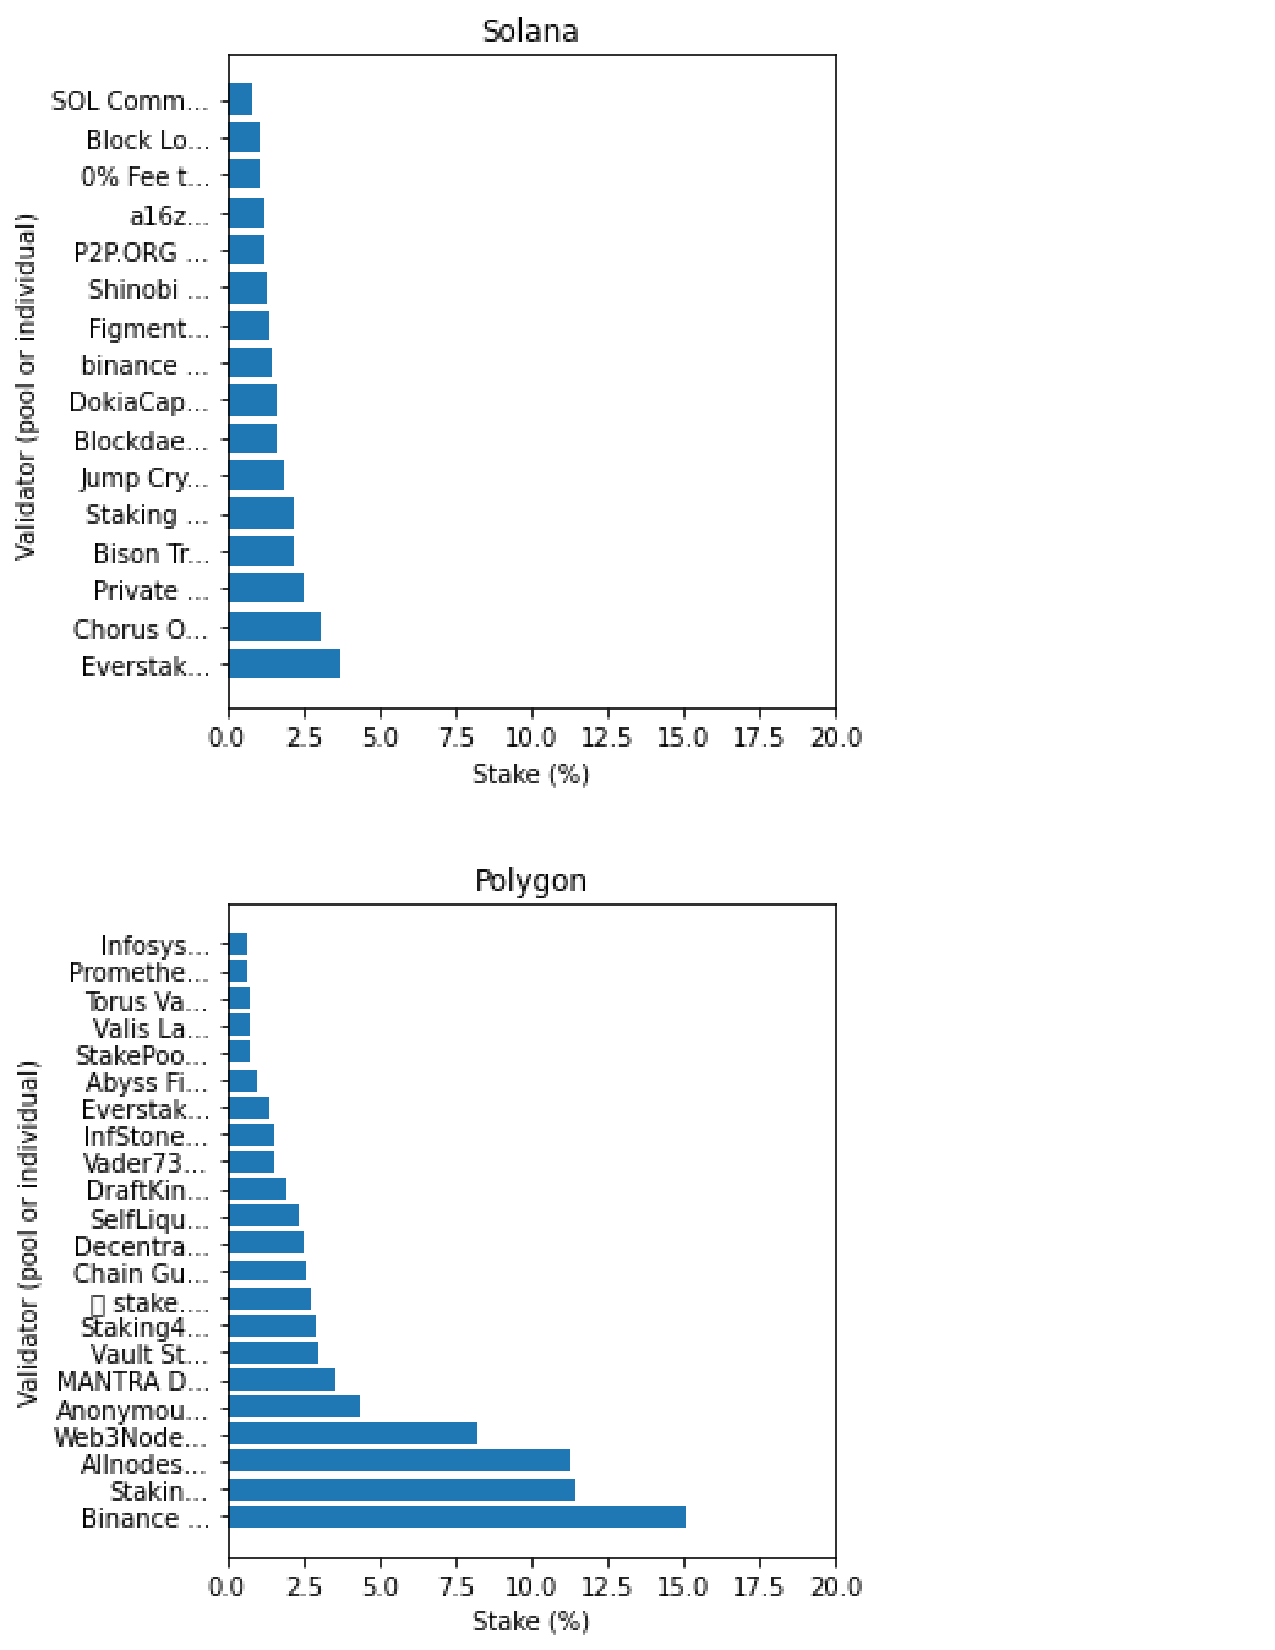
\includegraphics[width=3in]{figures/NetworkCentrality.pdf}
    \caption{Top 25 validators on Solana and Polygon \cite{solana_validators_www.validators.app} \cite{polygon_web_wallet_v2} (as of 27/03/22) shown against their percentage stake in the network. A less "bottom-heavy" graph indicated better distribution/decentralization as more validators are utilised. This shows Solana is far more distributed than Polygon with its top node staking 3.7\% of the network total while Polygon's top node stakes over 15\% of the network total.}
    \label{fig:networkcent}
\end{figure}

It is essential to be conscious of the degree of decentralization of a network. For example, one only has to look to the most popular decentralized game in the world (Axie Infinity \cite{whitepaper_axie_infinity}) to see the repercussions of having just 8 validators backing their network. The 51\% attack of Axie's Ronin network in April 2022 \cite{community_alert:_ronin_validators_compromised} lost users over \$600 million of various tokens. This demonstrates that it is key to find a healthy compromise between the speed and throughput offered by centralization and security and trust offered by decentralization.

The ideal blockchain for our work would have a good balance of speed (transaction confirmation time), throughput (TPS), wide distribution (well-rounded stake profile) and, VRF support. 

Speed and throughput speak for themselves as the number one critique of real-time DApps (like any sort of game) compared to traditional apps is their responsiveness, or rather, lack thereof. Thus, eliminating any bottleneck is key. 

Secondly, wide distribution means makes it more difficult for validators to collaborate and perform a 51\% attack on the network. While this would jeopardise all DApps on the network, a high-stakes iGaming casino would obviously be a primary target if there was a significant amount stored in its bank.

Finally, VRF support is rather self-explanatory - games of chance require randomness and randomness that is susceptible to attack (like hashing block alone data) undermines the principle of a fair, trustless casino.

\begin{table}[!h]
    \centering
    \renewcommand{\arraystretch}{1.3}
    \caption{Overview of a fees on current blockchains to build near real-time DApps that rely on verifiable randomness as of early 2022. VRF fees are given excluding gas fees incurred when invoking the random function.}
    \label{tab:blockfees}
    \begin{tabular}{c | c c}
        \hline\hline
        Blockchain & Transaction Fee (Transfer) & VRF Fee \\ 
        \hline
        Ethereum & 0.000546 ETH & 0.25 LINK\\
         & = 1.41 USD & = 4.26 USD \\
        \hline
        Avalanche & 0.001 AVAX & N/A\\
        &  = 0.09271 USD & \\
        \hline
        Solana & 0.000005 SOL & N/A\\
         &  = 0.00056 USD & \\
         \hline
        Polygon & 0.00000004 MATIC & 0.0001 LINK \\
         & = 0.0000000672 USD & = 0.001704 USD \\
        \hline\hline
    \end{tabular}
\end{table}

\begin{table}[!h]
    \centering
    \renewcommand{\arraystretch}{1.3}
    \caption{Overview of speed and throughput of the blockchains given in table \ref{tab:blockfees}. Throughput is given in expected peak transactions per second (TPS) if it has not been reached in practice.}
    \label{tab:blocktimes}
    \begin{tabular}{c | c c c c}
        \hline\hline
        Blockchain & Block time (s) & Peak Throughput (TPS) \\ 
        \hline
        Ethereum & $\sim$13.5 & 10-15\\
        Avalanche & 2 & 3400\\
        Solana & 0.4 & 65000\\
        Polygon & 2.2 & 7000\\
        \hline\hline
    \end{tabular}
\end{table}

As shown in tables \ref{tab:blockfees} and \ref{tab:blocktimes}, no blockchain fulfills all our criteria perfectly. Thus, we opted to use Polygon as our blockchain of choice to build GlassCasino due its well-roundedness in relation to all these categories and inherent security and strong ties to Ethereum as covered in Section \ref{sec:polygon}.

Another, less quantifiable, factor in selecting our blockchain was also its popularity and therefore the richness of its package ecosystem. Polygon supports every practically every mainstream technology that Ethereum supports to write, deploy, manage, and monitor smart contracts as well as a vast library of pre-written battle-tested implementation of common data structures or other systems.

\begin{figure}[!h]
    \centering
    \includegraphics[width=3.4in]{figures/polygon_ecosystem.jpg}
    \caption{A snapshot of the vast Polygon ecosystem \cite{polygon_matic_(@0xpolygon)_twitter} which, as shown, heavily overlaps with that of Ethereum thus offering excellent tooling, standards, and community discussion.}
    \label{fig:polygoneco}
\end{figure}

\subsection{Smart Contracts Overview}
Most smart contracts are usually written in a high-level language called Solidity \cite{solidity_programming_language} which is a classic curly-braced language. This language makes building large-scale maintainable projects viable for developers as the EVM can only execute bytecode of simple operations i.e. \texttt{XOR}, \texttt{ADD}, or some more complex but integral cryptographic hash functions like \texttt{KECCAK256} \cite{10.1007/978-3-642-38348-9_19}.

We used Remix \cite{verma2021study} IDE using Solidity to write and system test all of our contracts due to its numerous extensions to test for common security vulnerabilities, gas estimation and one-click deploy to a locally emulated blockchain.

For local development we used Ganache \cite{truffle_suite_ganache} to run a locally emulated Ethereum-like blockchain. This is excellent for rapid prototyping due to its instantaneous block times and full transaction history view.

Deploying a contract in a fault-tolerant manner is rather unwieldy. This is because a large contract costs a large amount of gas to deploy and may take multiple blocks for full confirmation due to a deployment being a very large transaction in of itself. Therefore we used a CLI tool called Truffle \cite{truffle_suite_truffle} to write migrations. These migrations are effectively deployment code that keeps track of its own status on the blockchain itself. We write a small deployment chain to deal with some edge cases and post-deployment operations which are covered later.

\subsection{EVM Event Logs}
\label{sec:evmlogs}
Before covering specific game contracts it is important to understand event logging on EVM-based blockchains. EVM bytecode defines five \texttt{LOG} operators to write records to any logging nodes. Each record consists of [0, 4] topics.

Topics are just any piece 256-bit data the developer of the contract wants logged. Solidity reserves one topic for the event/contract name. For example, take the following event definition from our roulette smart contract:
\begin{center}
    \texttt{event OutcomeDecided(uint256 outcome);}
\end{center}
Each time this event is emitted the EVM will invoke the \texttt{LOG2} operator to store the tuple (\texttt{KECCAK256('OutcomeDecided')}, outcome) to the global blockchain event logs.

These event logs can be queried by topic very quickly by using Bloom filters \cite{bloom1970space}. Included in the query result will be the transaction hash of the transaction that emitted the event and this can be used to extract further information like a timestamp or a block number.

This is excellent for DApp development where the state of the app (UI, logic etc.) often depends on past state and current blockchain state as its obviously not viable to record all relevant topics in some ever-expanding array in the blockchain's persistent state.

A trick this work utilises is block number caching. This is applicable when a developer wants all events $A$ that have been logged since the last event $B$ was logged. This is achieved by storing the block number $n$ on the persistent state of the blockchain when $B$ is logged and then limiting the query of $A$ to [$n + 1$, current block number]. 

\subsection{Dice}
The dice game available on GlassCasino is Chuck-a-Luck as mentioned earlier. It is a classic, simple game of chance with a relatively small house edge. A game is played as follows:
\begin{enumerate}
    \item Player selects a number in the range [1, 6].
    \item Three 6-sided dice are rolled randomly.
    \item Player is payed out if one or dice matches their roll, if none match they have lost.
\end{enumerate}

The simple games have made this game popular for many years and the adjustable payout rates have made it a casino-favourite for years. Classic rules dictate a single match is paid at 2:1 odds, two matches are paid at 3:1 while a triple match is casino-dependent.

\begin{table}[!h]
    \centering
    \renewcommand{\arraystretch}{1.3}
    \caption{Table of expected returns for the casino depending on the odds given for a triple match in Chuck-a-Luck\cite{chuck_luck_wizard_of_odds}.}
    \label{tab:chuckaluck}
    \begin{tabular}{c c}
        \hline\hline
        Payout for a Triple & House Edge \\ 
        \hline
        3:1 & 7.87\% \\
        4:1 & 7.41\% \\
        5:1 & 6.94\% \\
        6:1 & 6.48\% \\
        7:1 & 6.02\% \\
        8:1 & 5.56\% \\
        9:1 & 5.09\% \\
        10:1 & 4.63\% \\
        11:1 & 4.17\% \\
        12:1 & 3.7\% \\
        \hline\hline
        
    \end{tabular}
\end{table}

We opted for a payout of 10:1 and set the house edge to a fixed 5\% for simplicity's sake and to force immutability once the game is deployed to the blockchain. This is because , as described in Section \ref{sec:chainlink}, the VRF waits for 10 block confirmations between the request for randomness and its fulfillment. Therefore a mutable house edge could be changed by the house to an unfair extreme when a big enough game is started but before it concludes, granted they pay enough gas to get their transaction confirmed promptly. 

While this could be circumvented with locks on the manipulation of the odds, upper and lowers bounds et cetera it is overly complex and would against the tenet of writing legible, understandable contracts that can be trusted.

Developing the Dice contract presented a few challenges. The first of these comes from how the VRF contract works. First, our dice contract puts in a request for randomness and (given the contract has enough LINK) will get an ID of that request. This is because $\sim$10 blocks later the VRF contract will invoke the \texttt{fulfillRandomness} method of our dice contract with that ID. We must therefore maintain a mapping of player address to ID as to not mix games together. 

This does present an interesting idea of rolling randomness though so games can be fulfilled in less than 10 blocks but this is not explored in this work.

The second issue came, once again, from the \texttt{fulfillRandomness} function. ChainLink recommends consuming almost no gas in the function. Therefore, we tried maintaining a second map of players to their completed games and using \texttt{fulfillRandomness} to just write to this map and nothing more. However, this introduced a usability issue wherein players would need to invoke a transaction to claim their winnings, costing time and money (in gas fees). Also, we would need to maintain a third map to of user addresses to their game IDs to validate claim requests as legitimate.

However, an alternative option is possible. As established earlier, writing a value to non-volatile storage on the blockchain is very costly (20,000 gas to write a new value). ChainLink expects you do to this thus we can conclude we have at least this much gas to implement a less cumbersome method of prize distribution. Due to the implementation of our central bank, updating a user's balance costs 2,900 gas. Therefore we have $\sim$17,100 gas to calculate winnings based on the random result passed in.

Fortunately, calculating winnings can be implemented as a pure function meaning it doesn't read or write to any non-volatile state in the blockchain and is therefore cheaper. Next, the single random value from the VRF must be expanded out to three random values [1,6] fairly, to represent each die in Chuck-a-Luck. This can also be done in a pure function by rehashing the random value encoded with the index of the die (mod 6) + 1.

\begin{figure}[!h]
    \centering
    \includegraphics[width=3in]{figures/ChuckALuck.sol.png}
    \caption{UML class diagram of the \texttt{ChuckALuck} smart contract.}
    \label{fig:chuckuml}
\end{figure}
\subsection{Roulette}
The version of roulette implemented in this work follows a simplified European-style rule set. The wheel has just one zero giving a house edge of 2.7\%. The assignment of dividends to the owner is more simple than Chuck-a-Luck as all bets can simply be given to the owner when the wheel lands on the zero. There are just four bet types: odd, even, black, red. However, this is easily extensible.

Our implementation of the roulette smart contract, unlike the dice game, uses a vulnerable form of random number generation discussed earlier; hashing block data. This was done for simplicity and speed to implement as well to serve as a benchmark for just how unfortunately slow ChainLink VRF is in practice.

The roulette contract also has a few other minor differences from a single-player game like dice. Namely, we must account for an upper amount of bets available in a single round. This is done to reduce gas cost for users as writing to an dynamic array costs 4x as much gas. Secondly, there must be some trusted party to actually 'spin' the roulette wheel at a steady frequency. This is discussed further in Section \ref{sec:house}.

\begin{figure}[!h]
    \centering
    \includegraphics[width=3in]{figures/Roulette.sol.png}
    \caption{UML class diagram of the \texttt{Roulette} smart contract.}
    \label{fig:rouletteuml}
\end{figure}

\subsection{Central Banking}
\label{sec:bank}
Our initial design had each game's smart contract implement its own internal bank. This internal bank obviously requires elevated permissions that should not be afforded to any other user i.e. the ability to create or delete chips. Thus an internal bank where the contract itself is the only entity that can perform these actions seemed an ideal solution.

However, when building a second game a key usability problem arose; each user would have a different amount of chips on each table. This means if a user wins $x$ chips on game $i$ they cannot use their winnings on game $k$ without first withdrawing the $x$ chips to their wallet and then re-depositing them to the internal bank of game $k$. This is overly cumbersome and slow.

\begin{figure}[!h]
    \centering
    \includegraphics[width=3.6in]{figures/PreCentralBank.drawio.pdf}
    \caption{A diagram of a game-independent, internal banks as initially implemented and designed. This clearly demonstrates the inherent usability issue as users must jump through many hoops to withdraw their winnings and play another game.}
    \label{fig:precentralbank}
\end{figure}

The obvious solution here is to de-couple the banking logic from the game logic and maintain a list of games in a central bank that should be allowed to add or subtract funds.

\begin{figure}[!h]
    \centering
    \includegraphics[width=3.4in]{figures/CentralBank.drawio.pdf}
    \caption{Demonstration of how the game contracts and central bank contract interact with eachother and in relation to the user.}
    \label{fig:centralbank}
\end{figure}

Figure \ref{fig:centralbank} obviously presents a far less cumbersome experience for the end-user but introduces the issue of a central authority; the bank. This directly goes against the grain of what the underlying objective of this work.

The solution we implemented was a roles-based permission system allowed us to maintain trustlessness despite now having a central authority. 

This was achieved with an extension of OpenZeppelin's \texttt{AccessControlEnumerable} contract \cite{access_openzeppelin_docs}. OpenZeppelin is an extensively-tested, open-source repository of commonly used utilities for smart contracts and thus serves as an excellent resource for building out robust, maintainable systems.

The contract we specifically utilise here; \texttt{AccessControlEnumerable}, allows addresses to hold arbitrarily created roles defined by the contract developer. Each role has an administrator role that can add or remove users from its child role. Addresses can be a member of infinitely many roles. The enumerable aspect of the contract is a simple extension allowing iteration over all addresses that hold a given role.


\begin{figure}[!h]
    \centering
    \includegraphics[width=2.2in]{figures/AccessControl.drawio.pdf}
    \caption{General structure of the \texttt{AccessControl} roles. This shows the reliance on Solidity's \texttt{mapping} data structure allowing the mapping of an infinite input space to a finite output space. In the boolean case here any address not present in the mapping will default to false i.e., the user does not hold that role.}
    \label{fig:accesscontrol}
\end{figure}

Transactions defined in the contract can specify that they require the caller of the method to hold a specific role or else it will revert i.e., it will not mutate the state of the contract on the blockchain. This is key for us as we want to protect the methods of the bank that create or delete funds so only the games and nobody else can perform these actions. Then, since we assume the game code to be safe and fair - we maintain trustlessness.

To achieve this, we define two roles in the central bank; \texttt{ADMIN} and \texttt{OPERATOR}. In the contract's constructor (the code that is run once in its lifetime at deploy time) we set \texttt{ADMIN} as the super-role of \texttt{OPERATOR}. This means any address holding the \texttt{ADMIN} role can allocate any address the \texttt{OPERATOR} role at any time. 

Initially, the only address holding either role is the contract deployer as defined in the contract's constructor. They hold the \texttt{ADMIN} role. This means that they can then deploy a game contract with a reference to the deployed bank contract's address and allocate the game contract's address the \texttt{OPERATOR} role in the bank. This creates the two-way link we need where:
\begin{enumerate}
    \item The stand-alone bank contract must have a set of \texttt{OPERATOR} addresses who can manipulate funds (the game contract addresses) \textbf{AND}
    \item The game contract must have a reference to the address of the bank contract in order to call the methods that manipulate the funds
\end{enumerate}

Once all games have been deployed and tested the deployer should renounce their \texttt{ADMIN} role and thus no one will hold this role. This can be verified via enumeration as introduced earlier. Renunciation of the \texttt{ADMIN} role permanently freezes the list of addresses that hold the \texttt{OPERATOR} role as there is no  \texttt{ADMIN}s to add or remove addresses from this role. With this action, just like Figure \ref{fig:precentralbank}, the user only needs to trust the code of the game and the bank as no one other address has the ability to create or destroy funds.

In a development/testing environment however, it may desirable to allow the hot-swapping of games and thus on development networks or builds, the deployer can skip their renunciation of \texttt{ADMIN} and add/remove games in the future. This should never be the case in a production app though as there is a serious security risk of the \texttt{ADMIN} allocating themselves or a malicious contract the \texttt{OPERATOR} role, allowing them to empty the bank's real balance into their wallet.

\begin{figure}[!h]
    \centering
    \includegraphics[width=3in]{figures/DeployChain.drawio.pdf}
    \caption{Flowchart of our migration chain. It's important to note that each rectangular box represents a distinct migration step and is committed to the \texttt{Migrations} contract set up in the initial step. This means if the flow is interrupted for any reason (e.g. running out of gas) the deployment is restarted at that step after remedying the interruption.}
    \label{fig:deploychain}
\end{figure}

Another final step that is not technically part of the migration chain is the verification of contract source code on polygonscan \cite{polygonscan}. This is a web-based block explorer for the Polygon network which allows users to query any block number or hash, transaction hash, wallet address or, contract address and easily read all available, relevant information on the queried item. 

Polygonscan provides an API to upload contract source code in Solidity and compiler parameters (software version, optimizer passes etc.). This will be compared against the EVM bytecode stored on-chain and if its a match the verified human-legibible Solidity code will be stored on the contract's block explorer page. This work takes advantage of this API to further bolster the transparent nature of the casino.

\subsection{House Server}
\label{sec:house}
The house server is made up of two connected components; a websocket server and a blockchain-connected scheduler. Both of these components are written in Node.js.

Firstly, it is vital to establish how to interact with any state on the blockchain like balances, signing transactions or viewing contract state. This is done by making RPC (Remote Procedure Call) requests to an RPC API node. There two types of RPC nodes; public general use and developer cloud-hosted. General use nodes have a lower rate limit, do not require an API key and are typically for users to connect their wallet apps to the blockchain. Cloud-hosted nodes handle higher throughput, have a faster response time and can allow for access control. This access control can limit what contracts the node will allow interactions with or IP-based rules.

The option of self-hosting an RPC node was not explored in this work due its immense cost in time and money with a negligible performance edge. Instead, GlassCasino uses an RPC node provided by Alchemy \cite{why_use_alchemy_alchemy_documentation}. 

Integration with Alchemy is seamless and instantly offered speed improvements of multiple seconds over a general public RPC node like Polygon-RPC \cite{your_instant_rpc_gateway_to_polygon} which we originally used.

However, interacting with the RPC nodes directly is unnecessarily difficult. Instead, most developers utilise a library to abstract away the raw RPC method names, HTTP requests and packaging of operands. GlassCasino uses ethers.js \cite{ethers.js} for the house server and the web app.

\begin{figure}[!h]
    \centering
    \includegraphics[width=1.8in]{figures/HouseServer.drawio.pdf}
    \caption{Structure of how data from the blockchain is processed and use to authoritatively dictate game scheduling information and relay it to the web clients.}
    \label{fig:housserver}
\end{figure}

The scheduler is a simple timer implementation which listens for roulette bets and counts down a set interval to invoke the \texttt{play} transaction to 'spin the wheel'. It is designed to be online at all times and consume little to no compute power when no one is playing roulette. While this is not ideal as it adds a central authority to what is otherwise a completely distributed casino - it is a necessary component.

To schedule an event there must always be some timer. In classical centralized systems this is trivial to implement but it is unreasonable to expect validators to constantly run through a list of scheduled transactions at every iteration.

Projects like the Ethereum Alarm Clock Service \cite{ethereum_alarm_clock_documentation} work by providing upfront funds to cover future gas fees and a tip for invoking the function at a fixed interval. However, it still relies on an external network of task runners to be completing these tasks, thus it's not much better than a central task runner.

The existence of a central authority that control game flow does not completely undermine the trustless nature of the casino as the worst case scenario is that the admin can effectively hold users bets in limbo for which there is obviously no financial incentive.

A solution to this would be time-locking the \texttt{play} function by storing the timestamp in the contract's persistent state and verifying a certain amount of time has elapsed before any address can call it again. However, block timestamps are rather spaced out due to the multi-second block time of most networks and thus offer little precision which is important in building a robust UI. There also is still no guarantee that anyone would invoke the \texttt{play} transaction at all.
\subsection{Web App}
The final component to make this platform complete is, of course, some user interface to allow for interaction from the general public. Our work, in this regard, consists of a web application for maximum user reach. 

This is works well as the standard for DApps is to be web-based and rely on some kind of browser-installed (or, in the case of mobile devices; local app) wallet extension. The most well-known of these is MetaMask \cite{metamask:_the_crypto_wallet_gateway_to_web3_blockchain_apps} - a browser extension/mobile app wallet built for EVM-based blockchains like Ethereum or Polygon. 

The user interface (UI) itself was built with Vue 3 \cite{vue}. This allows the separation of the app into views which consist of components. Components can be easily re-used which is particularly useful when lots of instances of the same UI element exist independently from one another. For example, a fundamental component is that of a \texttt{BalanceBox} which takes a value in MATIC and formats it correctly with the token symbol after.

\begin{figure}[!h]
    \centering
    \includegraphics[width=1in]{figures/BalanceBox.jpg}
    \caption{Example of a \texttt{BalanceBox} with the extra 'Wallet' header used on GlassCasino to indicate a users current wallet balance without requiring the constant checking of their wallet provider.}
    \label{fig:balancebox}
\end{figure}

However, this component some extra functionality and styling because all values of ETH (or MATIC in our case) are given in wei. Every cryptocurrency supports the transfer of decimal values of itself. All cryptocurrencies specify how many decimals they support but the standard, set by ETH, is 18. 

However, it is obviously unwise to store it as a float on the machine itself due to the fact that rounding errors will have real financial ramifications.

Therefore, all libraries including ethers.js store currency values as 256-bit integers much like the EVM. This requires some special processing to convert to a string (as JavaScript does not support 256-bit integers) and round to $n$ decimal places.

Some components require the sharing of state. This is where a global state manager comes in. GlassCasino uses Vuex \cite{what_is_vuex_vuex}. This state contains:
\begin{enumerate}
    \item The global reference to the Alchemy RPC provider
    \item The transaction signer (given a wallet could be detected and its connection to GlassCasino was approved by the user)
    \item Extensive wallet detection and cookie-based memorisation of prior approval (this includes adding Polygon to the users wallet and switching networks if required)
    \item Reference to the \texttt{CentralBank} contract
    \item Reference to the currently open \texttt{Game} contract
    \item Current wallet \& \texttt{CentralBank} balances (given a signer exists), along with methods to refresh them
    \item WebSocket client to connect to the house server
    \item Dynamically updated game flow information from the house server
\end{enumerate}

We bind to the on-chain contracts by instantiating an instance of ethers.js's \texttt{Contract} utility class. In order to do this the application binary interface (ABI) is required along with the address of the deployed contract. Truffle saves this information in a JSON format each time the migration chain (figure \ref{fig:deploychain}) is ran. Thus, this JSON file is simply bundled into the webapp. 

\begin{figure}[!h]
    \centering
    \includegraphics[width=3.2in]{figures/BlockchainToUIBinding.drawio.pdf}
    \caption{Basic example of how the UI is bound to values fetched from Polygon's global state and how user interaction can will force these values to be refreshed thus updating the UI elements.}
    \label{fig:uibind}
\end{figure}

The rest of the UI is built up using local and global state and reusing component logic or styling as much as possible. The final work presented here consists of two full-screen views with some common elements between them like navigation bars.

\begin{figure}[!h]
    \centering
    \includegraphics[width=3.2in]{figures/RouletteView.jpg}
    \vspace{0.5cm} \ \\ 
    \includegraphics[width=3.2in]{figures/DiceView.jpg}
    \caption{Full views of the roulette UI (top) and the Chuck-a-Luck UI (bottom) on a standard 16:9 1920x1080 desktop monitor.}
    \label{fig:views}
\end{figure}

\begin{figure}[!h]
    \centering
    \includegraphics[width=2.3in]{figures/RouletteMobile.jpg}
    \caption{Full view of the roulette UI displayed at full-screen resolution on an iPhone XR (414px, 896px)}
    \label{fig:viewsmobile}
\end{figure}

As shown by figures \ref{fig:views} and \ref{fig:viewsmobile}; the web app is built to be responsive to viewports of all sizes and detect wallets on any mobile or desktop device. In the future, adding progressive web app (PWA) support would be desirable to create a native-like app feel with very little development overhead.

Some more interesting components to note are the roulette's: current bets and game history and Chuck-a-Luck's game history. All three of these components use event log querying to populate their UI with 'current bets' utilising the block number caching trick discussed in section \ref{sec:evmlogs}.

Each UI component that relates to a transaction (i.e. a specific bet or a game outcome) will also display a polygonscan URL along with it, allowing the user to verify the legitimacy of the game with one-click.

TODO include centralbank withdrawal screen here with some description if needed
% 2-3 pages for results
\section{Results}
\label{sec:results}
Our results are recorded with respect to the questions presented in section \ref{sec:introduction}, particularly we focus on measuring the technical viability of implementing a blockchain-backed online casino.

We break technical viability down into the following three sections:
\begin{enumerate}
    \item Speed
    \item Cost of operation (for the user and owner)
    \item Scalabity
\end{enumerate}

\subsection{Overall Platform Speed}
Our results pertaining to speed are split into two parts to measure separately:
\begin{enumerate}
    \item Smart contract speed
    \item Client speed (initial load, download size \& responsiveness)
\end{enumerate}

We measure smart contract execution speed by executing the most important transaction on each of our smart contracts $n$ times and timing how long it takes for confirmation. These results are displayed in figure \ref{fig:txspeeds}.

\begin{figure*}[h]
    \centering
    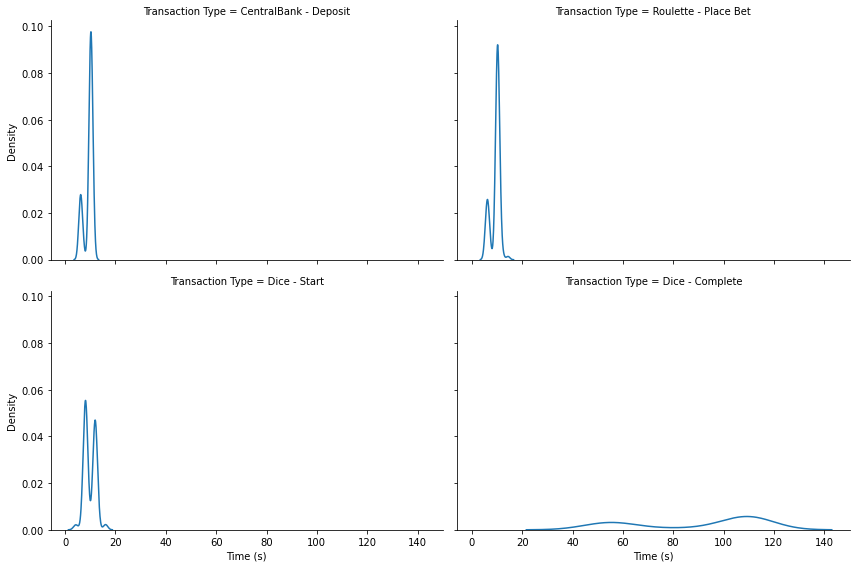
\includegraphics[width=6in]{figures/ContractTimings.png}
    \caption{Distribution of timings of entry-point transactions for each of our smart contracts. These were measured on the Polygon Mumbai test network with automatic gas fee estimation from ethers.js.}
    \label{fig:txspeeds}
\end{figure*}

To measure client app performance we utilise Google's WebPageTest.org \cite{webpagetest} to record bundle size (i.e. how much data the user must download to load a page), render progress, and other omitted metrics. We plot these results against two other similar apps (one decentralized, one not) as benchmarks.

\begin{figure}[!h]
    \centering
    \includegraphics[width=3.3in]{figures/VisualProgress.png}
    \caption{Visual progress graph of three gamblings web apps including GlassCasino. Measured on Firefox v98 for desktop, in Germany using a standard cabled internet connection (5000 Kbps down/1000 Kbps up, 28ms latency).}
    \label{fig:visprog}
\end{figure}

Speed index is defined as the area above each line in figure \ref{fig:visprog}:

\begin{equation}
    \int_{0}^{end} 1 - \frac{VC}{100}
\end{equation}

We calculate the corresponding speed indices for these web apps in table \ref{tab:speedindices}:

\begin{table}[!h]
    \centering
    \caption{Speed indices of the same three web apps as \ref{fig:visprog} and under the same test conditions.}
    \label{tab:speedindices}
    \begin{tabular}{c | c}
        \hline\hline
        Web App & Speed Index (ms) \\ 
        \hline
        bc.game & 1601 \\
        GlassCasino & 1609 \\
        Croissant Games & 18272 \\
        \hline\hline
    \end{tabular}
\end{table}

Finally, we find each web app's bundle size (the total size of JavaScript files, images, HTML and other documents downloaded when loading a page):

\begin{table}[!h]
    \centering
    \caption{Bundle sizes of the same three web apps as \ref{fig:visprog} and under the same test conditions.}
    \label{tab:bundlesizes}
    \begin{tabular}{c | c}
        \hline\hline
        Web App & Bundle Size (KB) \\ 
        \hline
        bc.game & 6035 \\
        GlassCasino & 399 \\
        Croissant Games & 17638 \\
        \hline\hline
    \end{tabular}
\end{table}

\subsection{Cost of Operation}
First we calculate the 'guzzle' rate of each game, This rate measures how many units of gas are used per minute by a given contract. Block explorers like polygonscan will list the top gas guzzlers and spenders. Guzzle rate (gas per second) is defined as follows for a set of transaction $T : |T| = k$ that occurred over $s$ seconds.
\begin{equation}
    G/s = \frac{\sum_{i=1}^{k} GasUsed(T_{i})}{s}
\end{equation}

The following tables show measured gas costs for important transactions on each smart contract (i.e. $GasUsed(T_i)$). These were measured using a locally deployed Ganache blockchain and the truffle command line tool. The contracts were compiled with Solidity 0.8.7 with 200 optimizer passes.

\begin{table}[!h]
    \centering
    \caption{Table of gas fees for the write transactions of the central bank smart contract.}
    \label{tab:bankgasfees}
    \begin{tabular}{c | c}
        \hline\hline
        Method & Gas Used \\ 
        \hline
        Deposit (from 0) &  43848 \\
        Withdraw (to 0) & 38394 \\
        Deposit & 28848 \\
        Withdraw & 23394 \\
        \hline\hline
    \end{tabular}
\end{table}

\begin{table}[!h]
    \centering
    \caption{Table of gas fees for the write transactions of the roulette smart contract. We assume all betters have non-zero balances and that the contract has been deployed and used for a while (i.e. all relevant fields are no longer at their initial value of zero).}
    \label{tab:roulettegasfees}
    \begin{tabular}{c | c c}
        \hline\hline
        Method & Gas Used \\ 
        \hline
        PlaceBet & [55868, 90068] \\
        Play (0 betters) & $\sim$30948 \\
        Play ($n$ betters, $n$ losers) & 23302 + $\sim$3149$n$ \\
        Play ($n$ betters, $\geq$1 winner) & 30948 + $\sim$3149$n$ \\
        \hline\hline
    \end{tabular}
\end{table}

\begin{table}[!h]
    \centering
    \caption{Table of gas fees for the write transactions of the Chuck-a-Luck smart contract. These results were measured on Polygon's Mumbai test network as the Chuck-a-Luck implementation uses ChainLink VRF.}
    \label{tab:dicegasfees}
    \begin{tabular}{c | c}
        \hline\hline
        Method & Gas Used \\ 
        \hline
        Play &  [178286, 212486] \\
        \hline\hline
    \end{tabular}
\end{table}

\begin{figure}[!h]
    \centering
    \includegraphics[width=3in]{figures/RouletteGuzzle-cropped.pdf}
    \caption{Simulated guzzle rate of the roulette contract. We assume a maximum bet count of 128, 45 second rounds, and a gas fee of 70 gwei (giga-wei) per unit of gas.}
    \label{fig:playguzzle}
\end{figure}

\begin{figure}[!h]
    \centering
    \includegraphics[width=3in]{figures/ChuckALuckGuzzle-cropped.pdf}
    \caption{Simulated guzzle rate of the Chuck-a-Luck contract. We assume a VRF fee of 0.0001 LINK per call, a MATIC to LINK exchange rate of 0.09541955, and a gas fee of 70 gwei per unit of gas.}
    \label{fig:chuckguzzle}
\end{figure}


\subsection{Scalability}
Scalability, is heavily correlated with the gas guzzle rate of contracts. We know the smart contracts to be the bottleneck of the platform and thus measure their scalability. We calculate this by taking the total block gas limit of Polygon (20 million gas / block) and the gas amounts presented in tables \ref{tab:roulettegasfees} and \ref{tab:dicegasfees} to visualise network utilisation against the transaction throughput supported. These results are shown in figures \ref{fig:roulettescalability} and \ref{fig:dicescalability}.

\begin{figure}[!h]
    \centering
    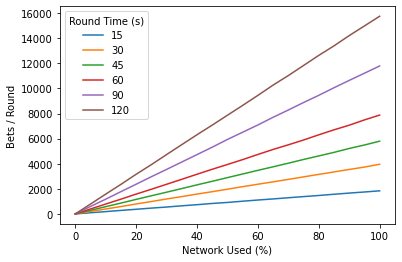
\includegraphics[width=3in]{figures/RouletteNetworkCongestion.png}
    \caption{Percentage of all gas used on the network (\%) against the number of betters that proportion of gas can support. This is repeated for various times between each wheel spin and includes the gas cost the owner pays to invoke the transaction to 'spin the wheel'.}
    \label{fig:roulettescalability}
\end{figure}

\begin{figure}[!h]
    \centering
    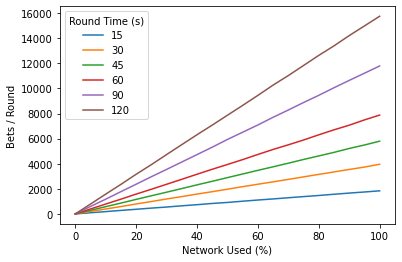
\includegraphics[width=3in]{figures/RouletteNetworkCongestion.png}
    \caption{TODO}
    \label{fig:dicescalability}
\end{figure}

%1 - 2 pages
\section{Evaluation}
We evaluate our work with respect to the three categories of technical viability presented in section \ref{sec:results}. However, we also consider the second question presented in section \ref{sec:introduction}; "To what degree can said implementation leverage the benefits offered by such technologies (i.e. provability, decentralization and security)?".

\subsection{Overall Platform Speed}
As \ref{fig:txspeeds} shows, transaction speeds of the three methods we wrote (first three, left to right) were consistent. However, their performance is still lacklustre with the majority of cases taking 6 or 10 seconds. Interestingly, we see large dips in the middle of all these distributions. This occurs as a transaction must be placed into a block and blockchains all have a fixed block time. Therefore, it's very preferable to get into the earliest block possible which in our tests seems to occur $\sim$6 seconds from invoking the transaction.

These speeds are almost entirely dependent on outside factors like network congestion or how much gas over the average the user pays when invoking the transaction. However, even if all outside factors were in our favour a best-case scenario of $\sim$6 seconds is not good enough to hold user interest, as most users will mentally switch context when waiting more than a second, and usually quit out after 10 \cite{schofield2016meaningfully}.

Chuck-a-Luck's time to completion is abysmal due to the process of generating verifiable randomness as described in section \ref{sec:chainlink}. Secure, decentralized DApps that depend on randomness will require a more creative usage of VRFs until a better alternative presents itself as wait times of nearly two minutes are unacceptable for the modern internet user.

As for the web app; our fundamental goal with building was to build a light, performant platform to partially make up for the poor speeds of transaction confirmation on the blockchain.

The HTTP archive \cite{loading_speed_http_archive} performs a monthly measurement of speed indices of the top one million websites as ranked by themselves. In 2022 they found the median speed index of a page loaded on desktop to be 3500 ms.

GlassCasino's excellent score of 1609ms puts it just outside the 10th percentile which sits at 1533ms. The indistinguishable result from that of bc.game is also very promising as it is a staple centralized iGaming platform. Our work also outperformed Croissant Games by an order of magnitude in this metric.

Our bundle size of 399 KB also fairs favourably compared to the findings of the HTTP archive and the benchmark web apps we measured against. Not only is our work 44x lighter (download-wise) than its closest peer but sits comfortably within the 10th percentile as total bundle sizes which is 455.1 KB. 

\subsection{Cost of Operation}
Placing bets guzzles much more gas but the cost is spread across many users.

Smart contract speed almost entirely depends on the congestion of the Polygon network, the current set block time, and the gas fees paid and thus, is highly variable. However (real user conditions, compare blah blah).

TODO finish

\subsection{Scalability}
TODO compare against throughput and speed of traditional online slots/roulette 

\subsection{Decentralization and Security}
TODO

\section{Conclusion}
TODO suggest future work i.e. separate network for each game (maybe invoke Avalanche P chain) (but not a Ronin situation) (explore gaslessness presented by Croissant games) etc. etc.

TODO extensions: need to redeploy webapp when contracts are updated as the ABI is bundled in, PWA support, more games (poker is particularly interesting as it's PvP), remove reliance on house server, allow users to plug in their own contract addresses for further security

This section summarises the main points of this paper. Do not replicate the abstract as the conclusion. A conclusion might elaborate on the importance of the work or suggest applications and extensions. This section should be no more than 1 page in length.
\newpage
\bibliographystyle{IEEEtran}
\bibliography{IEEEabrv, references}

% that's all folks
\end{document}


